\documentclass{article}
\usepackage{fancyhdr}
\pagestyle{fancy}
\lhead{Progetto finale di Reti Logiche - A.A. 2019/2020}
\rhead{Weger Marco}
\cfoot{\thepage}

\usepackage{tikz} % Import the tikz package
\usetikzlibrary{automata} % Import library for drawing automata
\usetikzlibrary{positioning} % ...positioning nodes
\usetikzlibrary{arrows} % ...customizing arrows

\usepackage{float}
\usepackage{amsmath}
\usepackage{tabularx}

\tikzset{
->, % makes the edges directed
node distance=3cm, % specifies the minimum distance between two nodes. Change if necessary.
every state/.style={thick, fill=gray!10}, % sets the properties for each ’state’ node
initial text=$ $, % sets the text that appears on the start arrow
}

\usepackage{lmodern}
\usepackage[T1]{fontenc}
\usepackage{textcomp}

\usepackage[italian]{babel}

\addto\captionsitalian{
  \renewcommand{\contentsname}
    {Contenuto}
}

\usepackage{graphicx}
\usepackage[font=small,labelfont=bf]{caption} % Required for specifying captions to tables and figures
\usepackage{footmisc}

\begin{document}
\pagenumbering{gobble}
\title{Progetto finale di Reti Logiche}
\author{Weger Marco - Matricola n° 888201}
\date{Anno Accademico 2019/2020}
\maketitle

\tableofcontents

\newpage
\pagenumbering{arabic}
\section{Introduzione}
Per questo progetto mi sono posto l'obiettivo di descrivere un componente che rispetti le specifiche sia in pre sintesi che in post sintesi.
Ho voluto scrivere del codice di facile lettura e che si adatti in modo semplice e rapido a qualsiasi tipo di modifica del pattern e/o della dimensione della memoria e del suo contenuto (più dettagli verranno forniti in seguito).
Per quanto riguarda la frequenza di clock non sono andato alla ricerca di una massimizzazione in quanto la specifica fissa il periodo di clock a 100 ns.
\subsection{Obiettivi aggiuntivi}
Dopo essermi assicurato di rispettate le richieste della specifica fornita mi sono posto i seguenti obiettivi:
\begin{enumerate}
	\item Minimizzare il tempo trascorso dal momento che il segnale di start viene ricevuto al momento di invio del segnale di done;
	\item Disattivare il segnale di enable della memoria tra le varie esecuzioni;
	\item Descrivere un componente in grado di funzionare anche nel caso ci fossero reset asincroni durante l'esecuzione di una codifica;
	\item Rendere il componente adattabile ad un'eventuale modifica della lunghezza dell'indirizzo della cella di memoria tramite una costante;
	\item Rendere il componente adattabile ad un'eventuale modifica della dimensione di una singola cella di memoria tramite una costante (ADDR);
	\item Rendere il componente adattabile ad un'eventuale modifica del numero di elementi in una working-zone tramite una costante (WZ\textunderscore OFFSET);
	\item Rendere il componente adattabile ad un'eventuale modifica del numero di working-zone tramite una costante (WZ\textunderscore NUM).
\end{enumerate}
Al fine di raggiungere i sopracitati obiettivi ho assunto che l'indirizzo da codificare e l'indirizzo codificato vengano sempre salvati in successione in celle immediatamente consecutive all'ultimo indirizzo di working-zone (ad esempio se ci fossero 16 working-zone, RAM(16) conterrebbe l'indirizzo da codificare e RAM(17) l'indirizzo codificato).

Tutte le ottimizzazioni descritte in seguito sono state valutate sulla base dei dati forniti dalla specifica e non tengono conto dell'eventuale crescita sproposita delle costanti sopracitate.
\subsection{Obiettivo velocità}
La limitazione più stringente in termini di velocità è data dall'accesso alla RAM e dai suoi ritardi. Al fine di minimizzare i tempi di letture e confronti ho optato per un componente che al momento della lettura di una cella imposti contemporaneamente la successiva richiesta. In questo modo posso garantire l'esecuzione dei confronti tra l'indirizzo e le N working-zone in N+1 cicli di clock. Occorreranno poi 2 cicli di clock per la scrittura del dato codificato in memoria e la notificazione di elaborazione completata. Un ulteriorie ciclo di clock mi è servito a garantire che il segnale \textit{o\textunderscore en} non rimanga attivo tra un'esecuzione e la successiva.
Ricapitolando, nel caso pessimo in cui l'indirizzo letto non si trova in nessuna delle work-zone:
\begin{equation*}
T_\mathrm{esecuzione} = (N+1) \cdot T_\mathrm{clock}+3 \cdot T_\mathrm{clock}
\end{equation*}
Nella valutazione del tempo di esecuzione va preso in considerazione il fatto che il segnale di start potrebbe arrivare sul fronte di discesa del clock, qualora succedesse l'esecuzione ritarderà di $T_\mathrm{clock}/2$.
Nella specifica forntia l'esecuzione massima dovrà durare 1200 ns (nel caso in cui \textit{i\textunderscore start} fosse allineato al fronte di salita del clock), 1250 ns altrimenti.
\subsection{Obiettivo codice semplice e riutilizzabile}
Ho deciso di realizzare una macchina a stati finiti al fine di rendere il codice facilmente comprensibile ed eventualmente modificabile, anche parzialmente.
Tutti i segnali sono gestiti da un'unica entity ad eccezione di un contatore generico utilizzato per scandire le working-zone.
Le seguenti costanti garantiscono un alto livello di riutilizzabilità (tra parentesi i valori assegnati da specifica):
\begin{itemize}
	\item \textbf{SIZE\textunderscore MEM} (16): dimensione dell'indirizzo di memoria;
	\item \textbf{SIZE\textunderscore ADDR} (8): dimensione di una cella di memoria;
	\item \textbf{SIZE\textunderscore WZ} (4): estensione della singola working-zone;
	\item \textbf{COUNT\textunderscore WZ} (3): dimensione del vettore \textit{WZ\textunderscore NUM};
	\item \textbf{N\textunderscore WZ} (8): numero di working-zone.
\end{itemize}
Viene naturale notare la relazione tra \textit{COUNT\textunderscore WZ} e \textit{N\textunderscore WZ}, nonostante ciò ho voluto esplicatre costanti differenti in modo da far fronte a situazioni in cui il numero di working-zone non è potenza di 2.
\subsection{Funzionamento in sintesi}
Una soluzione che memorizza tramite registri i valori delle working-zone avrebbe migliorato i tempi di esecuzione compromettendo l'adattabilità del componente a situazione con un maggior numero di working-zone e/o una RAM più grande; pertando ho optato per scandire la memoria a ogni esecuzione.
La singola esecuzione di una codifica può essere descritta attraverso un numero finito di step (che poi diventeranno una macchina a stati finiti):
\begin{enumerate}
	\item Reset ed attesa del segnale di start (\textit{i\textunderscore start=1});
	\item Abilitazione della memoria e richiesta dell'indirizo da codificare (salvato in un registro);
	\item Richiesta della i-esima working-zone e confronto con l'indirizzo salvato, eventuale codifica e passaggio a step successivo (passo ripetuto per i compreso tra 0 e il numero di working-zone);
	\item Scrittura dell'indirizzo codificato in memoria;
	\item Invio segnale di elaborazione completata (\textit{o\textunderscore done=1}) e attesa feedback (\textit{i\textunderscore start=0}), il dato è disponibile fin dal momento in cui \textit{o\textunderscore done} viene portato a 1;
\end{enumerate}
\subsection{Note aggiuntive sulla specifica}
Non sono stati considerati casi di working-zone sovrapposte in modo parziale o totale. Il componente scandisce in modo sequenziale le working-zone quindi viene identifica come valida quella nell'indirizzo RAM più basso (la scansione parte dall'indirizzo 0).
Per la sintesi è stata scelta l'FPGA xc7a200tfbg484-1.

\noindent\rule{\textwidth}{0.5pt}
\newpage
\section{Architettura}
\subsection{Macchina a stati finiti}
Il funzionamento del componente è scandito dalla macchina a stati finiti in figura 1, la funzionalità di ogni singolo stato è descritta nella tabella 1.
La macchina è sincronizzata con il segnale \textit{i\textunderscore clk} e sensibile al segnale \textit{i\textunderscore start}.
\begin{figure}[H]
\centering % centers the figure
\begin{tikzpicture}
%RST,EN_MEM,GET_ADDR,WZ,W_MEM,DONE);
\node[state, initial, minimum size=1.8cm] (RST)  at (0,3) {$RST$};
\node[state, minimum size=1.8cm] (MEM) at (5,3) {$MEM$};
\node[state, minimum size=1.8cm] (ADDR) at (10,3) {$ADDR$};
\node[state, minimum size=1.8cm] (WZ) at (10,0) {$WZ$};
\node[state, minimum size=1.8cm] (WRITE) at (5,0) {$WRITE$};
\node[state, accepting, minimum size=1.8cm] (DONE) at (0,0) {$DONE$};
\draw (RST) edge (MEM);
\draw (MEM) edge (ADDR);
\draw (ADDR) edge (WZ);
\draw (WZ) edge node [midway, below] {ADDR in WZ} node[above, midway] {last WZ checked} (WRITE);
\draw (WRITE) edge (DONE);
\draw (DONE) edge (RST);
\draw (WZ) edge[loop right] node {others} (WZ);
%{ADDR in WZ or LAST WZ checked}
\end{tikzpicture}
\caption{macchina a stati finiti implementata.}
\label{fig:my_label}
\end{figure}
\begin{table}[H]
\begin{tabularx}{\textwidth}{|l|X|}
\hline
Stato&Descrizione\\ \hline\hline
RST&Stato di reset della macchina. Da qui partono eventuali rieseccuzioni senza reset. Tutti i segnali vengono settati al loro valore di default (compreso \textit{o\textunderscore done} che potrebbe trovarsi alto) e il componente si prepara a leggere il l'indirizzo da codificare. La memoria è disattivata.\\ \hline
MEM&Utilizzato esclusivamente per abilitare la memoria prima di iniziare le letture.\\ \hline
ADDR&L'indirzzo da codificare viene prelevato e salvato in un apposito registro. Il contatore che scandisce le working-zone viene resettato e la memoria viene preparata per la lettura della prima working-zone.\\ \hline
WZ&Unico stato ciciclico della macchina. La condizione di uscita dal ciclo  è il raggiungimento dell'ultima working-zone (caso in cui l'indirizzo non subirà modifiche)
oppure l'identificazione della working-zone di appartenza (indirizzo da codificare). Nell'ultima esecuzione dello stato la memoria viene preparata per la scrittura del dato (codificato o meno).\\ \hline
WRITE&Il segnale \textit{o\textunderscore we} viene alzato per permettere alla memoria di prelevare il dato (\textit{o\textunderscore we}).\\ \hline
DONE&Viene notificato il  termine dell'esecuzione tramite \textit{o\textunderscore done} per poi tornare nello stato RST in attesa di una nuova esecuzione.  \\ \hline
\end{tabularx}
\caption{stati della macchina a stati finiti implementata.}
\end{table}
\subsection{Schema funzionale}
Analizzando i componenti più significativi dello schema prodotto da Vivado si possono notare le seguenti informazioni:
\begin{itemize}
	\item il segnale \textit{o\textunderscore data} (il valore finale dell'elaborazione) è derivato da 3 multiplexer:
	\begin{itemize}
		\item \textbf{next\textunderscore addr\textunderscore i}: discrimina l'appartenza o meno alla working-zone;
		\item \textbf{next\textunderscore addr0\textunderscore i}: discrimina l'eventuale offset nella working-zone;
		\item \textbf{current\textunderscore addr\textunderscore i}: è comandato dall'enable della memoria;
	\end{itemize} 
	\item i segnali a singolo bit \textit{o\textunderscore done}, \textit{o\textunderscore en} e \textit{o\textunderscore we} sono gestiti dagli omonimi flip flop;
	\item la macchina a stati finiti è gestita da un registro a 3 bit (\textbf{current\textunderscore state\textunderscore reg});
	\item l'indirizzo da codificare è memorizzato in un registro di 7 bit (\textbf{current\textunderscore addr\textunderscore reg});
	\item tutti i flip flop utilizzati sono di tipo D;
	\item il multiplexer che governa il segnale \textit{o\textunderscore address} è gestito da segnali costanti ad eccezione dei bit che ne scandiscono i valori da 0 a 9 (\textbf{o\textunderscore address\textunderscore i\textunderscore \textunderscore 1}).
\end{itemize}
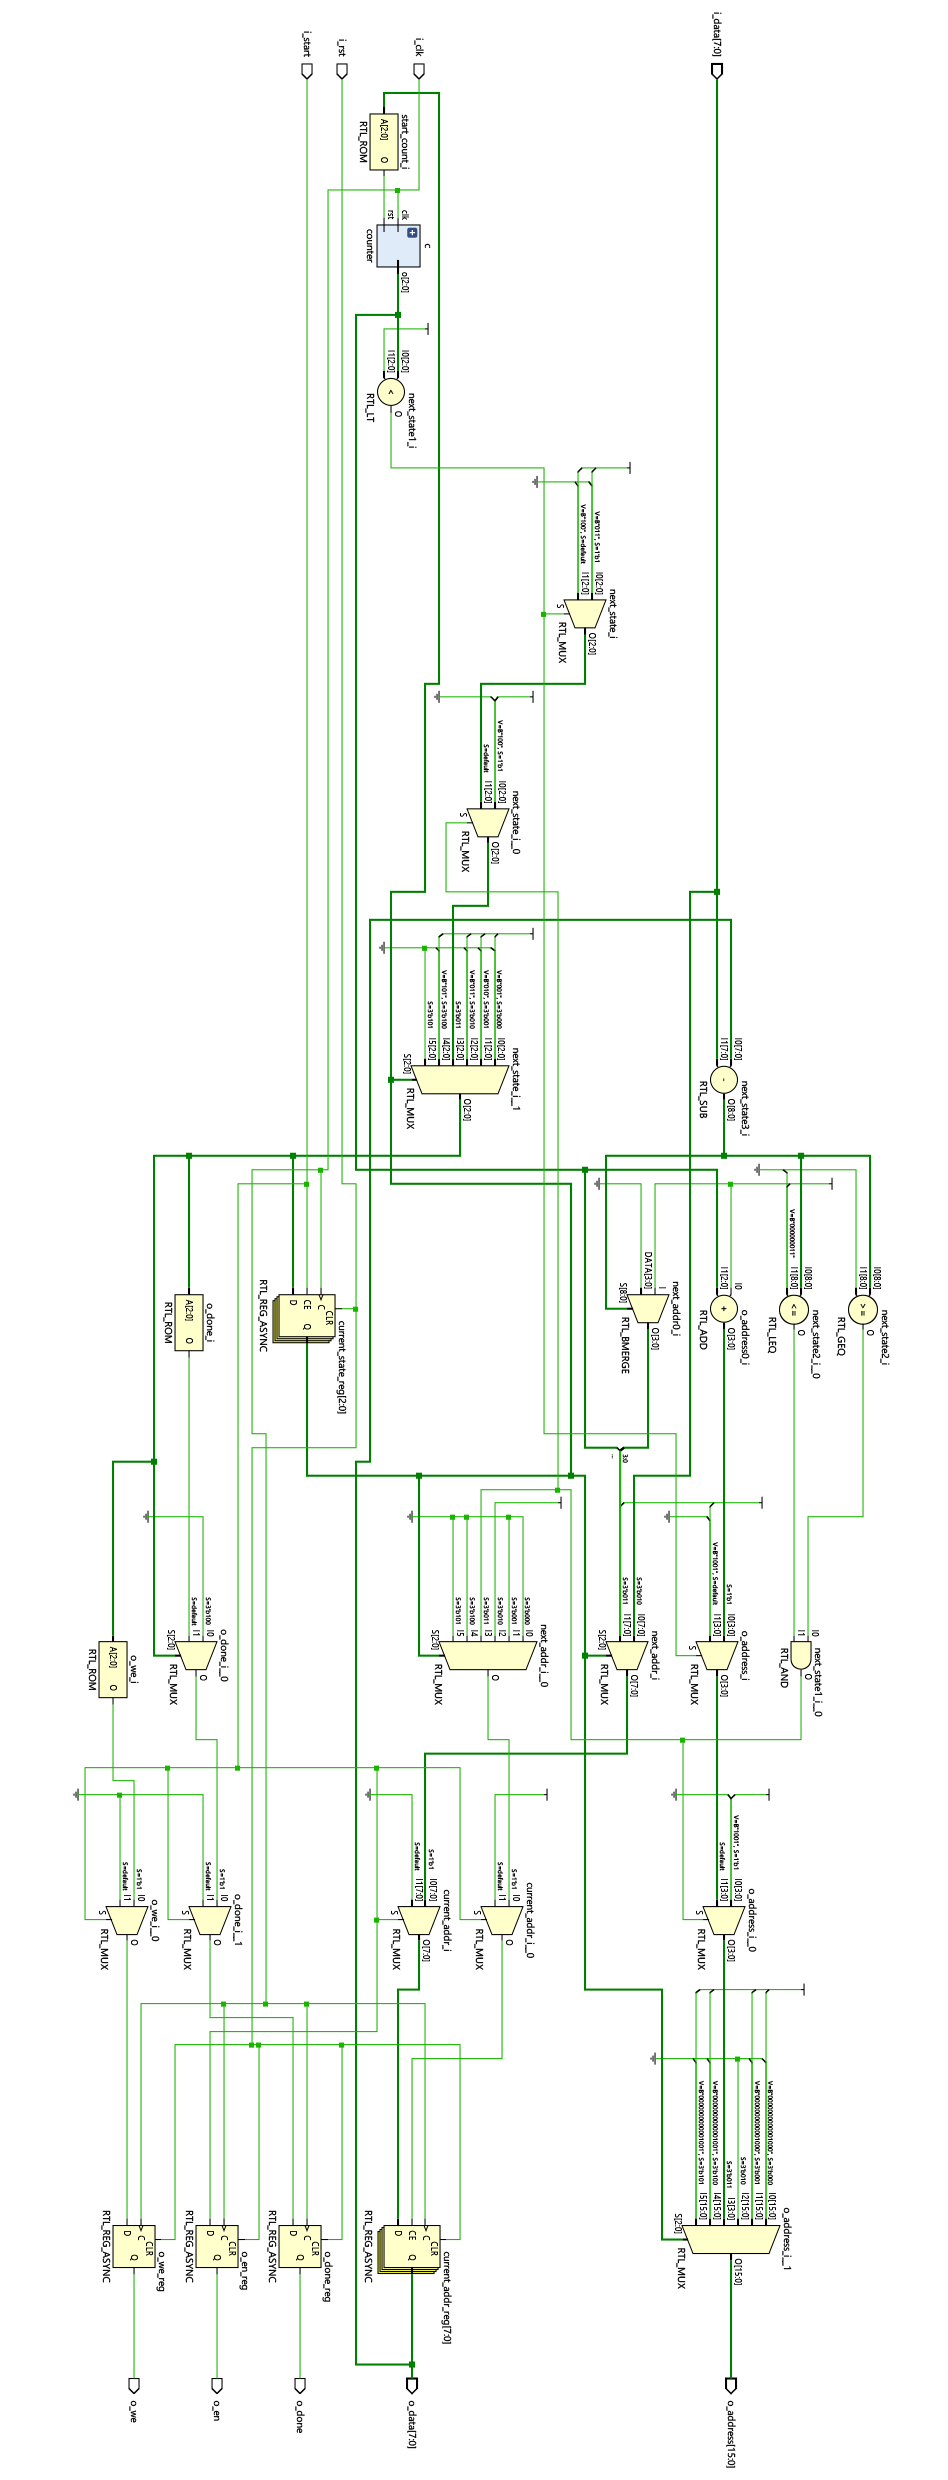
\includegraphics[height=0.92\textheight]{schematic.png}
\captionof{figure}{schema funzionale completo prodotto da Vivado.}

\noindent\rule{\textwidth}{0.5pt}
\newpage
\section{Sintesi}
\subsection{Registri sintetizzati}
Analizzando il report di sintesi e lo schema prodotto si può notare che gli stati della macchina sono codificati con la notazione "one hot" al fine di velocizzare le transizioni. Di seguito sono ricapitolati i registri sintetizzati.
\begin{table}[H]
\begin{tabularx}{\textwidth}{|l|l|l|X|}
\hline
N° bit&N° registri&Modulo&Contenuto\\ \hline\hline
8&1&main&Salvataggio dell'indirizzo da confrontare con le working-zone.\\ \hline
1&3&main&Gestione di segnali a singolo bit: \textit{o\textunderscore done}, \textit{o\textunderscore en}, \textit{o\textunderscore we}. \\ \hline
6&1&main&Codifica lo stato corrente della macchina secondo la notazione "one hot".\\ \hline
3&1&counter&Contatore a 3 bit usato per scandire le working-zone.\\ \hline
\end{tabularx}
\caption{registri sintetizzati e loro contenuto.}
\end{table}
\subsection{Area occupata}
Tramite le funzionalità di reportistica di VIVADO si possono analizzare il numero di LUT e di Flip Flop (a singolo bit) utilizzati.
\begin{table}[H]
\begin{tabularx}{\textwidth}{|X|X|X|X|}
\hline
Risorsa&Utilizzo&Disponibilità&Utilizzo in \%\\ \hline\hline
Look Up Table&30&134600&0,02229\\ \hline
Flip Flop&20&269200&0,00743\\ \hline
\end{tabularx}
\caption{area utilizzata dal componente in relazione all'FPGA citata nella sezione 1.5.}
\end{table}
\subsection{Report di timing}
La specifica non richiede la valutazione del Worst Negative Slack (WNS) di conseguenza verrà considerato massimo. Analizzando i test bench forniti ho notato che la RAM ha un ritardo di esecuzione (T\textsubscript{RAM}) di 1 ns. Dalle precendenti considerezanio segue il minimo periodo calcolabile:
\begin{equation*}
T_\mathrm{min} = T_\mathrm{RAM} + T_\mathrm{clock} - WNS \approx 1 ns + 100 ns - 100 ns = 1 ns 
\end{equation*}
Ne consegue la massima frequenza di clock: $f_\mathrm{max} = 1/T_\mathrm{min} \approx 1 Ghz$.
\subsection{Warnings}
Tutti i warning che si sono presentati durante lo sviluppo del componente sono stati risolti senza particolari difficoltà.
\subsection{Note aggiuntive sulla sintesi}
Per la sintesi ho usato la versione 2019.2 di XILINX VIVADO con i settaggi di default.

\noindent\rule{\textwidth}{0.5pt}
\newpage
\section{Simulazioni}
Oltre a testare il componente con i test bench forniti dalla specifica ho ritenuto opportuno valutare alcuni casi critici del funzionamento del componente (\textit{descritti nella sezione 4.3}).
\subsection{Indirizzo non nella working-zone (test bench fornito)}
Da questo test bench mi aspetto che tutta la memoria venga scandita e infine ADDR venga proposto senza variazioni.
Potremo inoltre valutare il tempo massimo per una singula esecuzione.
\subsubsection{Dati}
\begin{itemize}
	\item Working-zone: [4,13,22,31,37,45,77,91];
	\item ADDR: 42.
\end{itemize}
\subsubsection{Risultati in pre sintesi}
\captionof{figure}{valori dei segnali della entity durante la simulazione pre sintesi.}
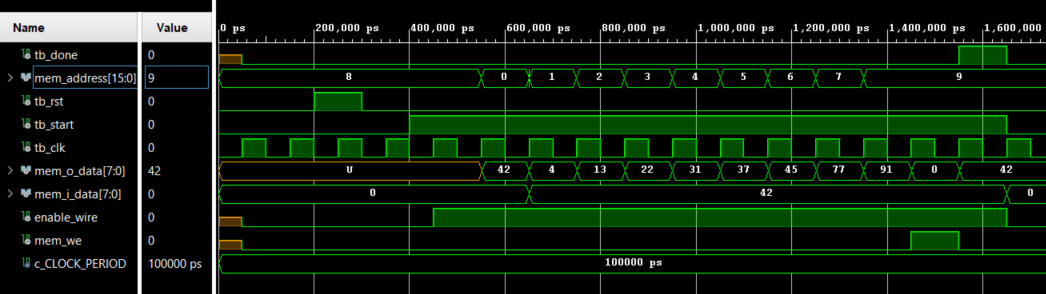
\includegraphics[width=\textwidth]{tb0.png}
Questo primo test mi conferma il corretto valore dei segnali in seguito al reset.
Trascuriamo per semplicità il fatto che il segnale di start arrivi sul fronte di discesa del clock e valutiamo i segnali ad ogni ciclo:
\begin{enumerate}
	\item Il segnale \textit{enable\textunderscore wire} viene alzato, mi aspetto che al prossimo clock venga caricato l'ADDR in \textit{mem\textunderscore o\textunderscore data};
	\item ADDR viene salvato nell'registro locale, alla memoria viene richiesta la prima WZ;
	\item Il confronto tra ADDR e WZ0 non è positivo, si passa al successivo;
	\item Il confronto tra ADDR e WZ1 non è positivo, si passa al successivo;
	\item Il confronto tra ADDR e WZ2 non è positivo, si passa al successivo;
	\item Il confronto tra ADDR e WZ3 non è positivo, si passa al successivo;
	\item Il confronto tra ADDR e WZ4 non è positivo, si passa al successivo;
	\item Il confronto tra ADDR e WZ5 non è positivo, si passa al successivo;
	\item Il confronto tra ADDR e WZ6 non è positivo, si passa al successivo;
	\item Il confronto tra ADDR e WZ7 non è positivo, i confronti sono terminati quindi \textit{mem\textunderscore address} viene correttamento portato a 9 (indirizzo dove deve scrivere) e in \textit{mem\textunderscore i\textunderscore data} viene messo 42 (ADDR non modificato);
	\item Il segnale \textit{mem\textunderscore we} viene alzato per scrivere in memoria il valore finale;
	\item La scrittura è terminata, si alza \textit{o\textunderscore done}.
\end{enumerate}
Una volta riportato \textit{tb\textunderscore start} a '0' il componente torna in modo corretto nella situazione iniziale (\textit{ulteriori test riguardanti esecuzioni in successione nella sezione 4.3}).
Il tempo di esecuzione, come mi aspettavo, è di 12 cicli di clock.
\subsubsection{Risultati in post sintesi}
\captionof{figure}{valori dei segnali della entity durante la simulazione post sintesi.}
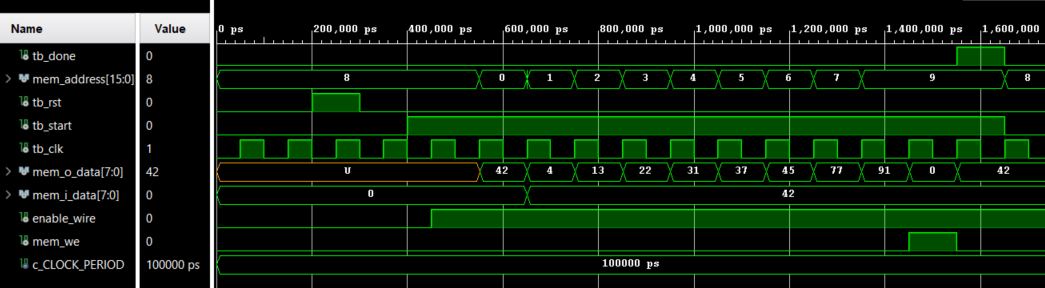
\includegraphics[width=\textwidth]{tb0-ps.png}

Non avendo latch e/o segnali indefiniti il test post sintesi è equivalente alla situazione in pre sintesi a meno di alcuni \textit{dont-care} che precedeno il reset iniziale (trascurabili).
\subsection{Indirizzo nella working-zone (test bench fornito)}
Da questo test bench possiamo verificare che i confronti con le working-zone e la codifica dell'indirizzo avvengano correttamente.
\subsubsection{Dati}
\begin{itemize}
	\item Working-zone: [4,13,22,31,37,45,77,91];
	\item ADDR: 33.
\end{itemize}
L'indirizzo si trova nella quarta working-zone quindi in output mi aspetto 180 (1-011-0100).
\subsubsection{Risultati in pre sintesi}
\captionof{figure}{valori dei segnali della entity durante la simulazione pre sintesi.}
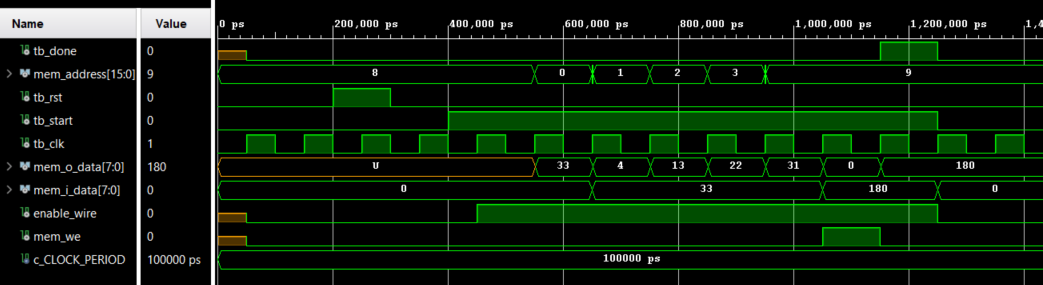
\includegraphics[width=\textwidth]{tb1.png}
Trascuriamo per semplicità il fatto che il segnale di start arrivi sul fronte di discesa del clock e valutiamo i segnali ad ogni ciclo:
\begin{enumerate}
	\item Il segnale \textit{enable\textunderscore wire} viene alzato, mi aspetto che al prossimo clock venga caricato l'ADDR in \textit{mem\textunderscore o\textunderscore data};
	\item ADDR viene salvato nell'registro locale, alla memoria viene richiesta la prima WZ;
	\item Il confronto tra ADDR e WZ0 non è positivo, si passa al successivo;
	\item Il confronto tra ADDR e WZ1 non è positivo, si passa al successivo;
	\item Il confronto tra ADDR e WZ2 non è positivo, si passa al successivo;
	\item Il confronto tra ADDR e WZ3 è positivo, \textit{mem\textunderscore address} viene correttamento portato a 9 (indirizzo dove deve scrivere) e in \textit{mem\textunderscore i\textunderscore data} viene messo 180 (ADDR nella quarta working-zone con offset 3);
	\item Il segnale \textit{mem\textunderscore we} viene alzato per scrivere in memoria il valore finale;
	\item La scrittura è terminata, si alza \textit{o\textunderscore done}.
\end{enumerate}
Una volta riportato \textit{tb\textunderscore start} a '0' il componente torna in modo corretto nella situazione iniziale (\textit{ulteriori test riguardanti esecuzioni in successione nella sezione 4.3}).
Il tempo di esecuzione è di 8 cicli di clock, quattro in meno rispetto al test bench precedenze dato che non sono stati necessari gli ultimi confronti.
\newpage
\subsubsection{Risultati in post sintesi}
\captionof{figure}{valori dei segnali della entity durante la simulazione post sintesi.}
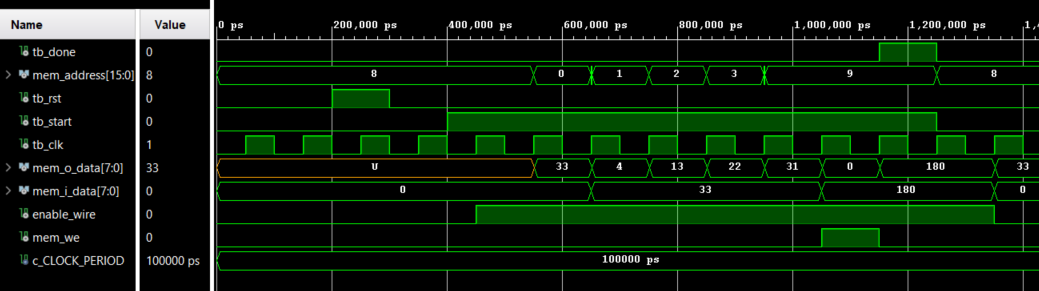
\includegraphics[width=\textwidth]{tb1-ps.png}
Non avendo latch e/o segnali indefiniti il test post sintesi è equivalente alla situazione in pre sintesi a meno di alcuni \textit{dont-care} che precedeno il reset iniziale (trascurabili).
\subsection{Altri test bench}
Ho realizzato ulteriori test al fine di verificare le seguenti situazioni:
\begin{itemize}
	\item ADDR nella prima working-zone (confine);
	\item ADDR nell'ultima working-zone (confine);
	\item ADDR nella working-zone con offset 0 (confine);
	\item ADDR nella working-zone con offset 3 (confine);
	\item riesecuzione di una codifica senza invio del segnale di reset;
	\item invio del segnale di reset nel mentre di un'esecuzione.
\end{itemize}
Tutti i test bench, compresi quelli nelle sezioni 4.1 e 4.2, hanno dato esito positivo sia in pre che in post sintesi.
I test bench sono stati infine eseguiti in post implementazione confermando i risultati precedenti.
Non sono state fatte ulteriori analisi sulla situazione in post implementazione.

\noindent\rule{\textwidth}{0.5pt}
\newpage
\section{Conclusione}
Ricapitolando ho descritto un componente con le seguenti caratteristiche:
\begin{itemize}
	\item funzionante in pre/post sintesi e in post implementazione;
	\item ottimizzato sotto il punto di vista dell'area utilizzata;
	\item ottimizzato sotto il punto di vista del tempo di esecuzione;
	\item altamente personalizzabile e configurabile mediante l'uso di costanti;
	\item utilizzo di LUT\footnote{Calcoli basati sulla dimensione della FPGA citata nella sezione 1.5\label{fn}}  par al 0,02229\%;
	\item utilizzo di FF\footref{fn} par al 0,00743\%.
\end{itemize}

\noindent\rule{\textwidth}{0.5pt}
\end{document}